
\documentclass[a4paper,12pt]{article}

\usepackage[utf8]{inputenc}
\usepackage[spanish]{babel}
\usepackage{amsmath, amssymb}
\usepackage{graphicx}
\usepackage{float}
\usepackage{booktabs}
\usepackage{xcolor}
\usepackage{listings}
\usepackage{caption}
\usepackage{fancyhdr}
\usepackage{hyperref}
\usepackage{tikz}

\hypersetup{
    colorlinks=true,
    linkcolor=blue,
    urlcolor=blue,
    pdftitle={Práctica 3 - ESP32},
}
% ---------- PREÁMBULO: arreglar comillas en listings (Thonny style) ----------
\usepackage[utf8]{inputenc}   % si no está ya
\usepackage[T1]{fontenc}      % mejor soporte de tipografías para PDFs
\usepackage{textcomp}         % símbolos de texto adicionales
\usepackage{upquote}          % comillas ' y " tipo ASCII en verbatim/listings

% Si usas babel con español, desactiva el shorthand de la comilla doble
\usepackage[spanish]{babel}
\shorthandoff{"}  % <<< evita que " sea un caracter activo (causa comillas invisibles)

% Colores inspirados en Thonny
\usepackage{xcolor}
\definecolor{thonnyKeyword}{rgb}{0.0,0.2,0.8}
\definecolor{thonnyComment}{rgb}{0.0,0.5,0.0}
\definecolor{thonnyString}{rgb}{0.7,0.12,0.12}
\definecolor{thonnyBackground}{rgb}{1.0,1.0,1.0}
\definecolor{thonnyBuiltin}{rgb}{0.5,0.0,0.5}
\definecolor{thonnyNumber}{rgb}{0.35,0.35,0.35}

% Declaración de lenguaje MicroPython (basado en Python)
\usepackage{listings}
\lstdefinelanguage{MicroPython}{
    morekeywords={
        False, True, None, and, as, assert, async, await, break, class, continue,
        def, del, elif, else, except, finally, for, from, global, if, import,
        in, is, lambda, nonlocal, not, or, pass, raise, return, try, while, with, yield
    },
    morekeywords=[2]{print,open,range,len,abs,int,float,str,dict,list,set,tuple},
    morekeywords=[3]{machine,network,time,urequests,utime,gc,Pin,ADC,PWM,UART,RTC,ESP32},
    sensitive=true,
    morecomment=[l]{\#},
    morestring=[b]",
    morestring=[b]',
}

% Configuración de listings con estilo Thonny (y upquote activo)
\lstset{
    language=MicroPython,
    backgroundcolor=\color{thonnyBackground},
    keywordstyle=\color{thonnyKeyword}\bfseries,
    keywordstyle=[2]\color{thonnyBuiltin},
    keywordstyle=[3]\color{thonnyKeyword!60!black},
    commentstyle=\color{thonnyComment}\itshape,
    stringstyle=\color{thonnyString},
    numberstyle=\tiny\color{thonnyNumber},
    basicstyle=\ttfamily\small,
    numbers=left,
    numbersep=6pt,
    frame=single,
    framerule=0.4pt,
    breaklines=true,
    breakatwhitespace=true,
    showstringspaces=false,
    tabsize=2,
    captionpos=b,
    columns=flexible,
    upquote=true     % importante para mostrar comillas rectas correctamente
}
% -------------------------------------------------------------------------


\title{Práctica N°3: Uso de base de datos FireBase en ESP32 con comunicación Wi-Fi}
\date{}

\begin{document}
\maketitle
\tableofcontents
\newpage

\section{Objetivos}

\subsection{Objetivo general}
Implementar y comprender el proceso completo de conexión entre una placa ESP32 y la base de datos en tiempo real de Firebase utilizando MicroPython, desde la configuración inicial del entorno hasta la ejecución del código de lectura y autenticación.

\subsection{Objetivos específicos}
\begin{itemize}
    \item Configurar la interfaz de desarrollo web y los servicios necesarios en Firebase para la comunicación con el ESP32.
    \item Establecer la conexión WiFi del microcontrolador y validar la autenticación mediante el uso del servicio \texttt{Firebase Auth REST API}.
    \item Comprender la estructura y funcionamiento del código en MicroPython que permite leer datos del nodo remoto de la base de datos.
    \item Analizar los mecanismos de reautenticación, manejo de errores y mantenimiento de conexión dentro del bucle principal del programa.
    \item Verificar el correcto intercambio de datos entre la placa y Firebase mediante la consola UART del entorno Thonny.
\end{itemize}

\section{Configuración de la base de datos Firebase}

Antes de ejecutar el programa en el ESP32, es necesario crear e integrar un proyecto en \textbf{Firebase Realtime Database}. Esta configuración permitirá almacenar y acceder a los datos que el microcontrolador leerá mediante el servicio REST. A continuación, se detallan los pasos a seguir desde la consola web de Firebase.

\subsection{Creación del proyecto en Firebase}

\begin{enumerate}
    \item Acceder a la página oficial de \texttt{https://firebase.google.com} e iniciar sesión con una cuenta de Google.
    \item En el panel principal, seleccionar \textbf{“Ir a la consola”} y luego hacer clic en \textbf{“Agregar proyecto”}.
    \item Asignar un nombre al proyecto, por ejemplo: \texttt{maestria-iiot-rppico}, y desactivar la opción de Google Analytics (no es necesaria para esta práctica).
    \item Presionar \textbf{“Crear proyecto”} y esperar a que se complete la inicialización.
\end{enumerate}

\begin{figure}[H]
    \centering
    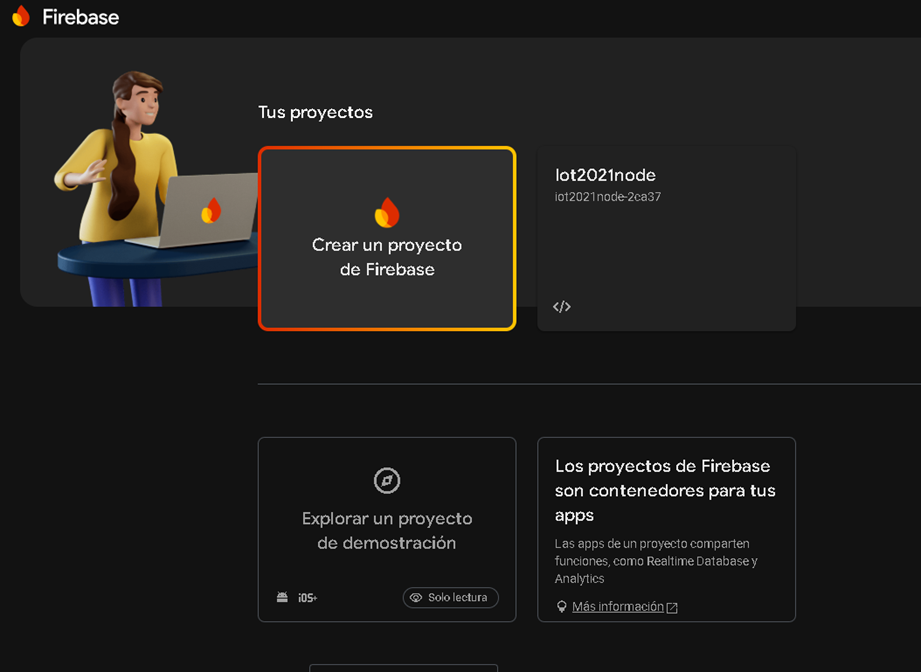
\includegraphics[width=0.8\textwidth]{FireBase/crear.png}
    \caption{Creación del nuevo proyecto en Firebase.}
\end{figure}

Este paso establece el entorno donde residirán los datos leídos por el ESP32. Cada proyecto de Firebase contiene servicios independientes, por lo que mantener un nombre descriptivo ayuda a identificar su propósito.

\subsection{Activación de la base de datos en tiempo real}

\begin{enumerate}
    \item En el menú lateral del proyecto, seleccionar la opción \textbf{“Base de datos”}.
    \item Elegir \textbf{“Base de datos en tiempo real”} y luego hacer clic en \textbf{“Crear base de datos”}.
    \item Seleccionar la ubicación del servidor (por ejemplo, \texttt{us-central1}) y escoger el modo \textbf{“Prueba”} para permitir temporalmente el acceso sin reglas estrictas de seguridad.
\end{enumerate}

\begin{figure}[H]
    \centering
    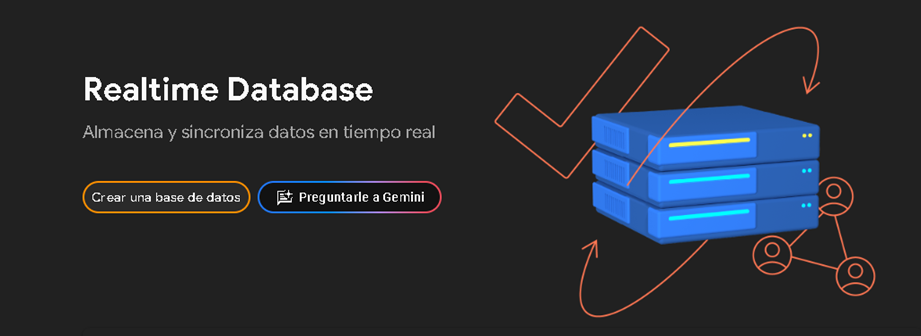
\includegraphics[width=0.8\textwidth]{FireBase/paso3.png}
    \caption{Inicialización del servicio Realtime Database.}
\end{figure}

\begin{figure}[H]
    \centering
    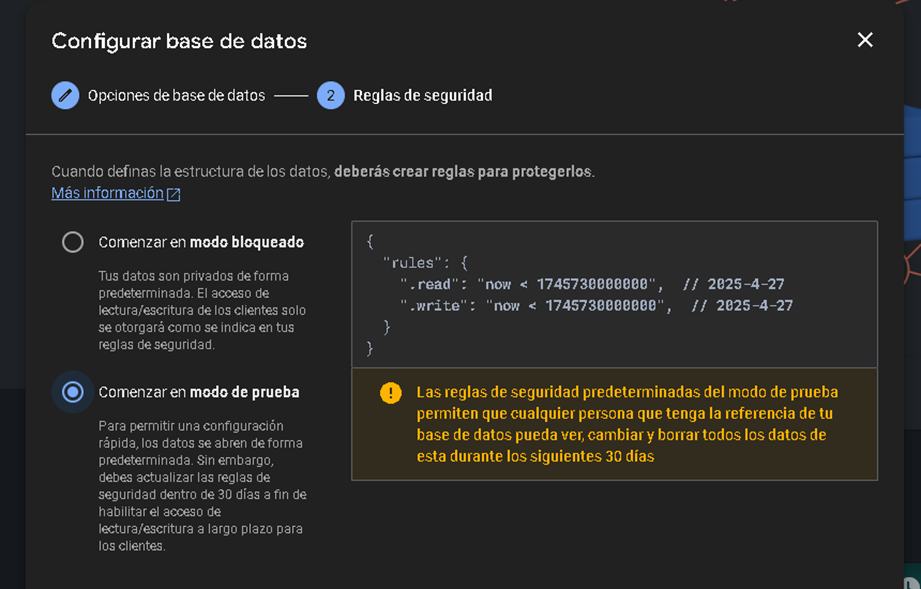
\includegraphics[width=0.8\textwidth]{FireBase/paso4.png}
    \caption{Inicialización del servicio Realtime Database.}
\end{figure}

El modo “Prueba” facilita la depuración inicial permitiendo operaciones de lectura y escritura sin autenticación. Sin embargo, en entornos productivos debe reemplazarse por reglas de acceso controlado mediante tokens de autenticación.

\subsection{Obtención de la URL del proyecto}

Al crear la base de datos, Firebase genera una URL única con el formato:

\begin{center}
    \texttt{https://<nombre-del-proyecto>.firebaseio.com/}
\end{center}

Esta dirección debe copiarse e insertarse en el archivo \texttt{main\_firebase.py} dentro de la variable \texttt{FIREBASE\_URL}.  
Es el punto de enlace que el ESP32 usará para consultar los datos del nodo remoto.

\begin{figure}[H]
    \centering
    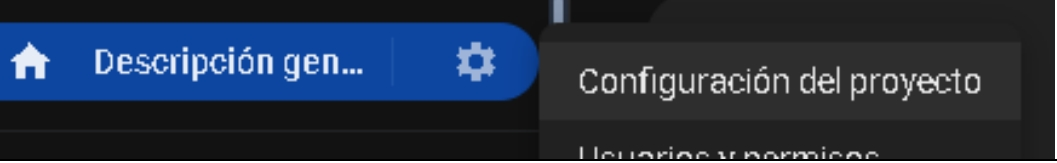
\includegraphics[width=0.8\textwidth]{FireBase/Config_api.jpeg}
    \caption{Obtención de la URL base de la Realtime Database.}
\end{figure}

\begin{figure}[H]
    \centering
    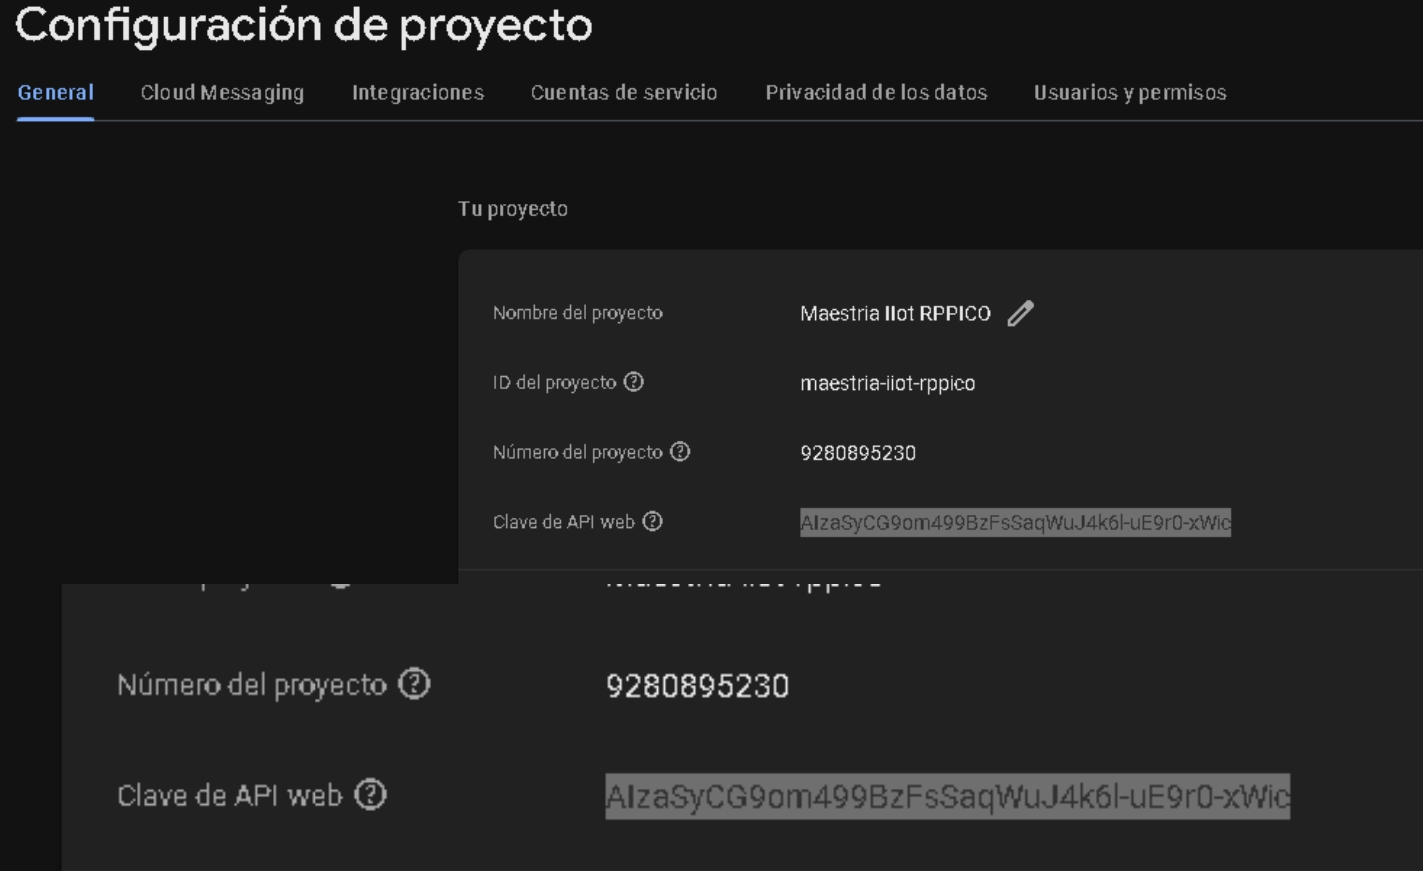
\includegraphics[width=0.8\textwidth]{FireBase/config_api2.jpeg}
    \caption{Obtención de la URL base de la Realtime Database.}
\end{figure}

\subsection{Configuración de autenticación por correo y contraseña}

\begin{enumerate}
    \item En el panel del proyecto, acceder al apartado \textbf{“Authentication”}.
    \item Hacer clic en \textbf{“Empezar”} y seleccionar el método \textbf{Correo electrónico / contraseña}.
    \item Activar este método y guardar los cambios.
    \item En la pestaña \textbf{Usuarios}, crear un nuevo usuario con correo y contraseña, por ejemplo:
    \begin{itemize}
        \item Correo: \texttt{usuario@ejemplo.com}
        \item Contraseña: \texttt{Paul2179}
    \end{itemize}
\end{enumerate}

\begin{figure}[H]
    \centering
    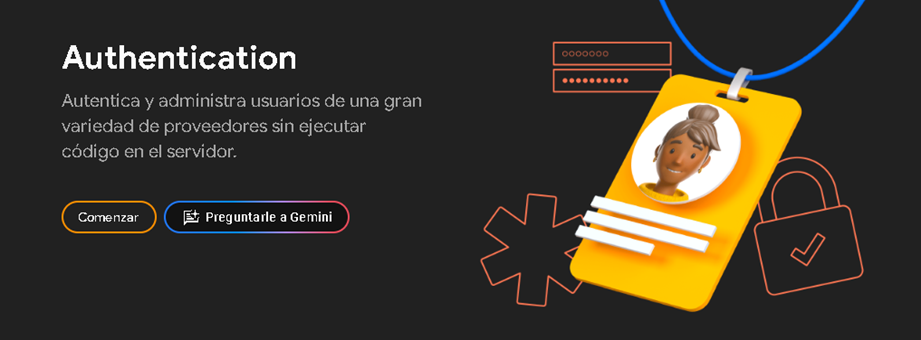
\includegraphics[width=0.8\textwidth]{FireBase/paso6.png}
    \caption{Habilitación del método de autenticación por correo y contraseña.}
\end{figure}

\begin{figure}[H]
    \centering
    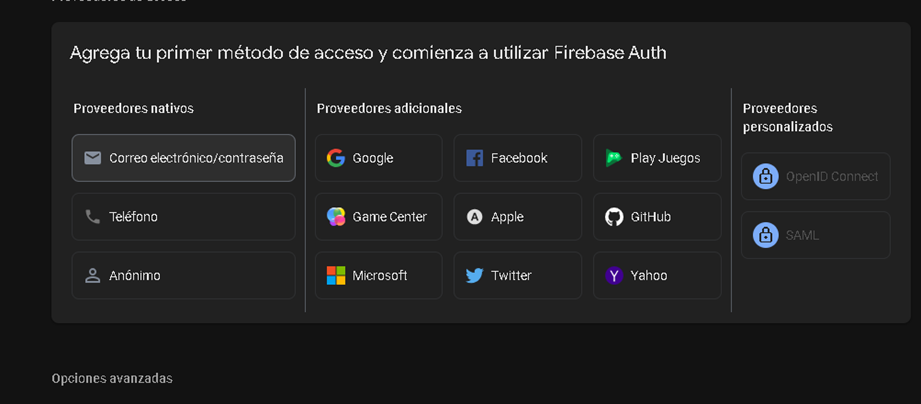
\includegraphics[width=0.8\textwidth]{FireBase/paso7.png}
    \caption{Habilitación del método de autenticación por correo y contraseña.}
\end{figure}

\begin{figure}[H]
    \centering
    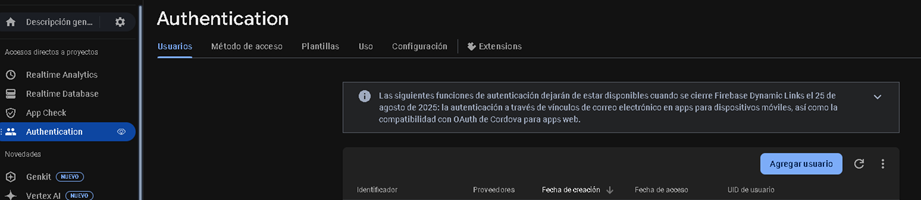
\includegraphics[width=0.8\textwidth]{FireBase/paso8.png}
    \caption{Habilitación del método de autenticación por correo y contraseña.}
\end{figure}

\begin{figure}[H]
    \centering
    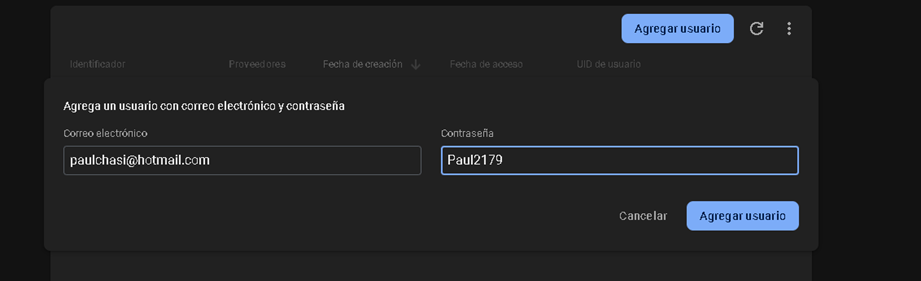
\includegraphics[width=0.8\textwidth]{FireBase/paso9.png}
    \caption{Habilitación del método de autenticación por correo y contraseña.}
\end{figure}

Esta credencial es la que permitirá que el ESP32 se autentique ante Firebase mediante la función \texttt{firebase\_auth()} en el código. El uso de tokens evita exponer directamente las credenciales en las solicitudes de lectura y escritura.

\subsection{Verificación de la estructura de datos}

Dentro del editor de la base de datos, se puede crear manualmente un nodo de prueba con el nombre \texttt{/random} y valores de ejemplo:

\begin{verbatim}
{
  "data": 25,
  "temperatura": 32
}
\end{verbatim}

\begin{figure}[H]
    \centering
    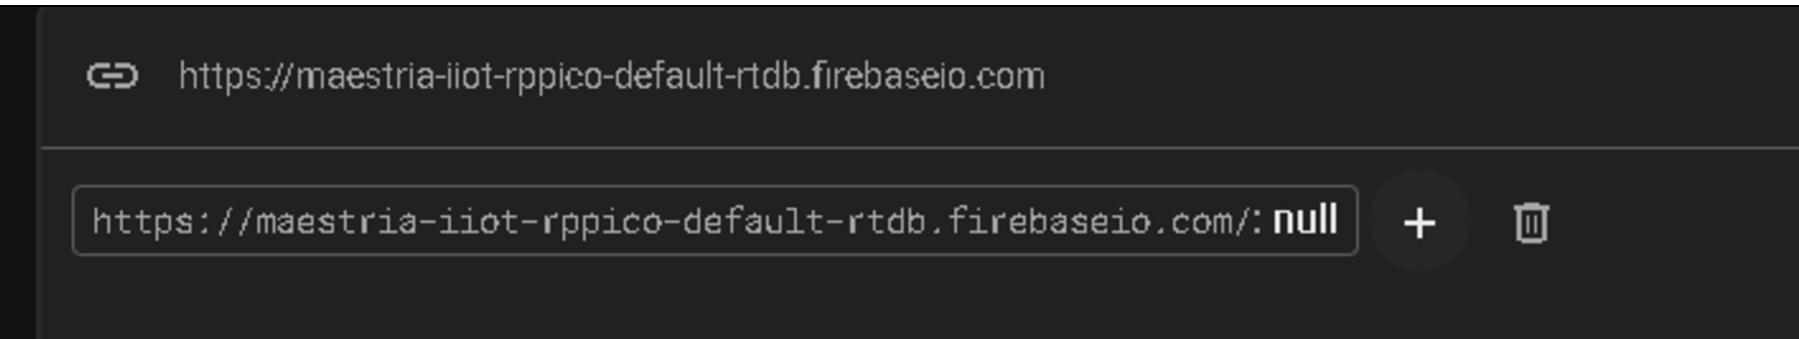
\includegraphics[width=0.8\textwidth]{FireBase/Datos_1.jpeg}
    \caption{Creación del nodo /random para pruebas de lectura.}
\end{figure}

\begin{figure}[H]
    \centering
    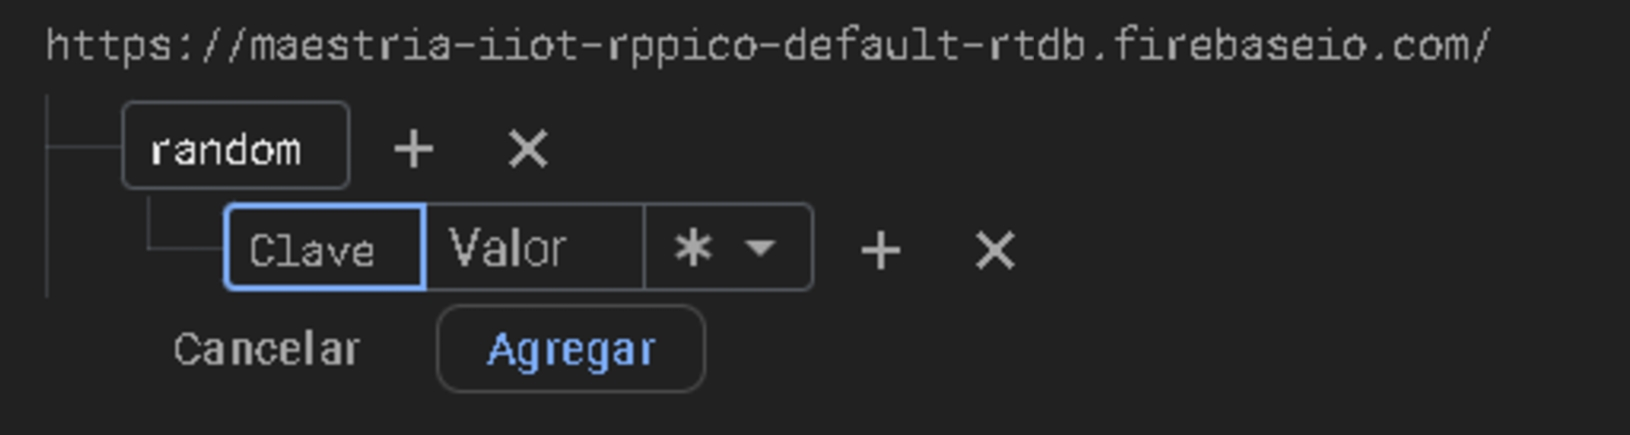
\includegraphics[width=0.8\textwidth]{FireBase/Datos_2.jpeg}
    \caption{Creación del nodo /random para pruebas de lectura.}
\end{figure}

\begin{figure}[H]
    \centering
    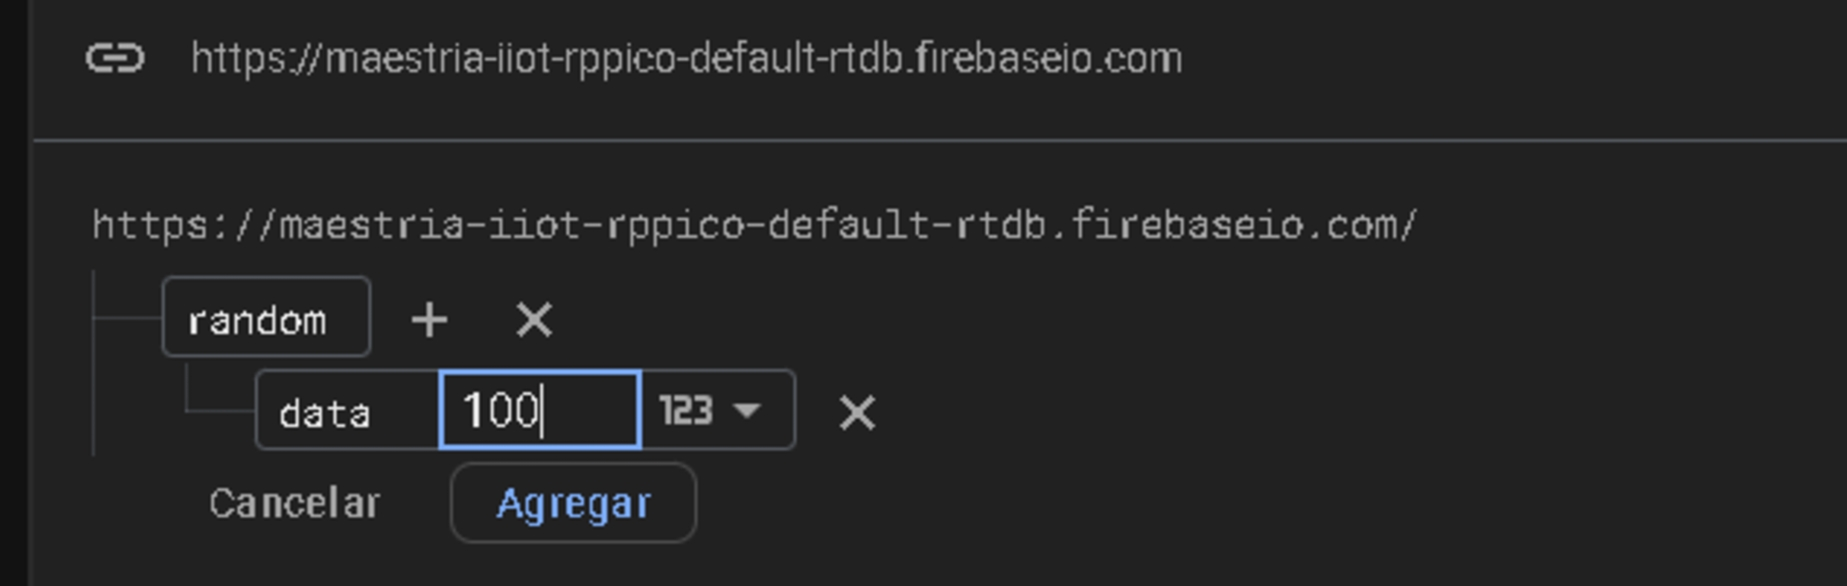
\includegraphics[width=0.8\textwidth]{FireBase/Datos_3.jpeg}
    \caption{Creación del nodo /random para pruebas de lectura.}
\end{figure}

\begin{figure}[H]
    \centering
    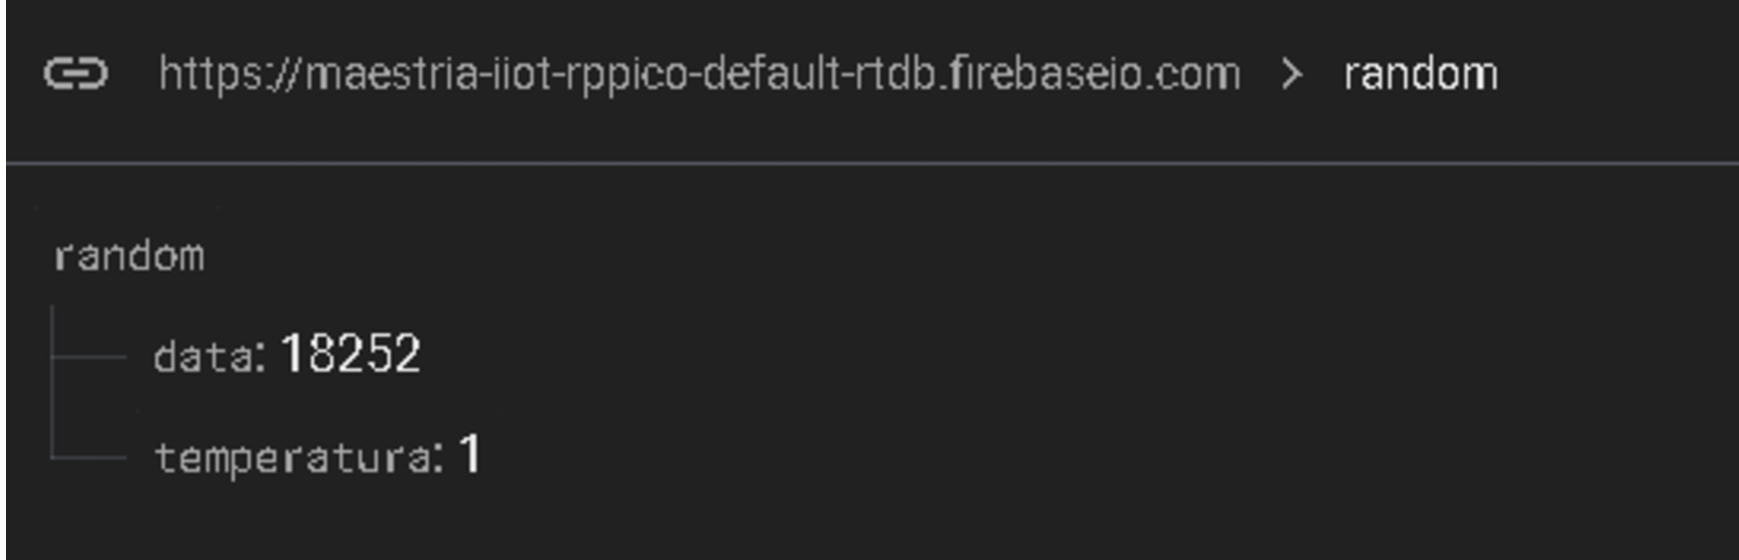
\includegraphics[width=0.8\textwidth]{FireBase/Datos_4.jpeg}
    \caption{Creación del nodo /random para pruebas de lectura.}
\end{figure}

Este nodo será el destino de las consultas REST que el microcontrolador realizará periódicamente.  
Si el código funciona correctamente, los valores almacenados aquí se mostrarán en la consola UART del entorno Thonny.



\section{Explicación del código}

A continuación se muestra el archivo completo \texttt{main\_firebase.py} que se utilizará en la práctica. Después del código, se explica cada sección.



\subsection{Código completo}

\begin{lstlisting}[language=Python,caption={main_firebase.py — código completo (MicroPython, ESP32)}]
# -*- coding: utf-8 -*-
# main.py ESP32 (MicroPython)
# Guarda este archivo directamente en la placa usando Thonny.

import network
import urequests as requests
import time
import gc

# =======================
# CONFIG (credenciales)
# =======================
WIFI_SSID = 'TU_SSID'
WIFI_PASSWORD = 'TU_PASSWORD'

FIREBASE_URL = 'https://maestria-iiot-rppico-default-rtdb.firebaseio.com/'
FIREBASE_EMAIL = 'usuario@example.com'
FIREBASE_PASSWORD = '********'
FIREBASE_API_KEY = 'AIzaSy***************'

# Intervalo de lectura en segundos (ajusta aqui)
POLL_INTERVAL = 3  # lectura cada 3 segundos

# =======================
# Variables internas
# =======================
id_token = None
wlan = None

# =======================
# Funciones
# =======================
def connect_wifi(timeout=15):
    #Conecta el ESP32 a la red WiFi. Lanza RuntimeError si falla.
    global wlan
    wlan = network.WLAN(network.STA_IF)
    wlan.active(True)
    if wlan.isconnected():
        print(" WiFi ya conectado. IP:", wlan.ifconfig()[0])
        return

    print(" Activando interfaz WiFi...")
    wlan.connect(WIFI_SSID, WIFI_PASSWORD)
    start = time.time()
    while not wlan.isconnected():
        if time.time() - start > timeout:
            raise RuntimeError(" Timeout: no se pudo conectar a WiFi")
        print(".", end="")
        time.sleep(1)
    print("\n WiFi conectado. IP:", wlan.ifconfig()[0])

def firebase_auth():
    """Autentica contra Firebase Auth REST y actualiza id_token global."""
    global id_token
    auth_url ="https://identitytoolkit.googleapis.com/
    v1/accounts:signInWithPassword?key={}".format(FIREBASE_API_KEY)
    auth_data = {
        "email": FIREBASE_EMAIL,
        "password": FIREBASE_PASSWORD,
        "returnSecureToken": True
    }
    try:
        print("Autenticando en Firebase...")
        resp = requests.post(auth_url, json=auth_data)
        if resp.status_code == 200:
            j = resp.json()
            id_token = j.get("idToken")
            if not id_token:
                print(" No se recibio idToken en la respuesta.")
                return False
            print(" Autenticacion exitosa.")
            return True
        else:
            print("Error auth (HTTP {}): {}".format(resp.status_code, resp.text))
            return False
    except Exception as e:
        print(" Excepcion durante auth:", e)
        return False
    finally:
        try:
            resp.close()
        except:
            pass
        gc.collect()

def read_firebase_data():
    """Lee el nodo /random.json con el idToken actual."""
    if not id_token:
        print(" No hay id_token - autenticate primero.")
        return None
    url = "{}random.json?auth={}".format(FIREBASE_URL, id_token)
    try:
        resp = requests.get(url)
        if resp.status_code == 200:
            data = resp.json() or {}
            # Impresion formateada
            print("\n" + "="*40)
            print(" DATOS DE FIREBASE (nodo /random)")
            print("="*40)
            print(" data     :", data.get("data", "N/D"))
            print(" temperatura:", "{}C".format(data.get("temperatura", "N/D")))
            print("="*40)
            return data
        else:
            print(" Error lectura (HTTP {}): {}".format(resp.status_code, resp.text))
            # Si token expiro, Firebase devuelve 401 o info similar -> retornar None para re-auth
            return None
    except Exception as e:
        print(" Excepcion en lectura:", e)
        return None
    finally:
        try:
            resp.close()
        except:
            pass
        gc.collect()

def main():
    global id_token
    try:
        connect_wifi()
    except Exception as e:
        print(" No se pudo iniciar WiFi:", e)
        return

    # Intentos de autenticacion (reintentar 2 veces)
    for attempt in range(3):
        if firebase_auth():
            break
        print(" Reintentando auth... ({}/{})".format(attempt+1, 3))
        time.sleep(2)
    else:
        print(" No se pudo autenticar en Firebase - abortando.")
        return

    print("\n Iniciando bucle de monitoreo (CTRL+C para detener)...")
    last_auth_time = time.time()
    AUTH_EXPIRY_SECONDS = 50 * 60  # reauth cada 50 min (ajustable)

    try:
        while True:
            data = read_firebase_data()
            if data is None:
                # Posible token expirado o error puntual: intentar re-autenticar una vez
                print(" Intentando re-autenticacion...")
                if not firebase_auth():
                    print(" Re-auth fallida. Esperando y reintentando mas tarde.")
                    time.sleep(5)
                else:
                    print(" Re-auth exitosa.")
            # Reautenticar periodicamente para evitar tokens caducados
            if time.time() - last_auth_time > AUTH_EXPIRY_SECONDS:
                print(" Reautenticando por tiempo transcurrido...")
                if firebase_auth():
                    last_auth_time = time.time()
            time.sleep(POLL_INTERVAL)
    except KeyboardInterrupt:
        print("\n Bucle detenido por usuario.")
    except Exception as e:
        print(" Error inesperado en main loop:", e)
    finally:
        try:
            if wlan:
                wlan.disconnect()
                wlan.active(False)
        except:
            pass
        gc.collect()
        print(" Fin.")

# =======================
# Ejecutar
# =======================
if __name__ == "__main__":
    main()
\end{lstlisting}

\newpage

\subsection{Explicación por secciones}

\subsubsection{Encabezado e \texttt{imports}}

\begin{lstlisting}[language=Python,caption={Imports y cabecera}]
# -*- coding: utf-8 -*-
# main.py ESP32 (MicroPython)
# Guarda este archivo directamente en la placa usando Thonny.

import network
import urequests as requests
import time
import gc
\end{lstlisting}

Primero se importan las bibliotecas necesarias: \texttt{network} para gestionar la interfaz WiFi, \texttt{urequests} (micro versión de requests) para realizar peticiones HTTP, \texttt{time} para temporización y \texttt{gc} para invocar el recolector de basura.

Se debe considera que en MicroPython el uso de memoria es limitado; por eso el código llama a \texttt{gc.collect()} en bloques \texttt{finally}. Cada petición HTTP y cada objeto JSON consume RAM.


\subsubsection{Configuración (credenciales y parámetros)}

\begin{lstlisting}[language=Python,caption={Variables de configuración}]
# =======================
# CONFIG (credenciales)
# =======================
WIFI_SSID = 'TU_SSID'
WIFI_PASSWORD = 'TU_PASSWORD'

FIREBASE_EMAIL = 'usuario@example.com'
FIREBASE_PASSWORD = '********'
FIREBASE_API_KEY = 'AIzaSy***************'
FIREBASE_URL = 'https://maestria-iiot-rppico-default-rtdb.firebaseio.com/'

# Intervalo de lectura en segundos (ajusta aqui)
POLL_INTERVAL = 3  # lectura cada 3 segundos
\end{lstlisting}

Se definen los parámetros necesarios para la práctica: credenciales WiFi, URL base de Firebase, API key y credenciales de autenticación (correo/clave), además del intervalo de muestreo.

\begin{itemize}
  \item \textbf{Seguridad:} no es buena práctica dejar credenciales en texto plano. En un entorno real conviene:
    \begin{itemize}
      \item mover credenciales a un archivo \texttt{secrets.py} (no subirlo al repositorio), o
      \item solicitar credenciales por consola/puerto serie, o
      \item usar variables de entorno (si el entorno lo permite).
    \end{itemize}
  \item \textbf{POLL\_INTERVAL:} escoger un intervalo mayor reduce consumo de red y CPU; en baterías conviene aumentar este valor.
\end{itemize}

\subsubsection{Variables internas globales}

\begin{lstlisting}[language=Python,caption={Variables internas}]
# =======================
# Variables internas
# =======================
id_token = None
wlan = None
\end{lstlisting}

Se definen las reservas globales para almacenar el \texttt{id\_token} de Firebase (token JWT devuelto por el servicio Auth) y el objeto \texttt{wlan} de la interfaz de red. El uso de variables globales facilita el diseño pero exige cuidado con concurrencia y estado; aquí el programa es secuencial, por lo que es aceptable.

\subsubsection{\texttt{connect\_wifi()}: conectar la placa a la red}

\begin{lstlisting}[language=Python,caption={Función connect\_wifi}]
def connect_wifi(timeout=15):
    """Conecta el ESP32 a la red WiFi. Lanza RuntimeError si falla."""
    global wlan
    wlan = network.WLAN(network.STA_IF)
    wlan.active(True)
    if wlan.isconnected():
        print(" WiFi ya conectado. IP:", wlan.ifconfig()[0])
        return

    print(" Activando interfaz WiFi...")
    wlan.connect(WIFI_SSID, WIFI_PASSWORD)
    start = time.time()
    while not wlan.isconnected():
        if time.time() - start > timeout:
            raise RuntimeError(" Timeout: no se pudo conectar a WiFi")
        print(".", end="")
        time.sleep(1)
    print("\n WiFi conectado. IP:", wlan.ifconfig()[0])
\end{lstlisting}

Mediante la interfaz WiFi en modo station, inicia la conexión y espera hasta que la conexión se establezca o ocurra un timeout.

\begin{itemize}
  \item \textbf{Timeout:} evita bloqueos indefinidos; el valor por defecto es 15 s.
  \item \textbf{Mensajes por UART:} se usan \texttt{print()} para informar al usuario — en la práctica esto se verá en la consola de Thonny.
\end{itemize}

\subsubsection{\texttt{firebase\_auth()}: autenticación contra Firebase}

\begin{lstlisting}[language=Python,caption={Función firebase\_auth}]
def firebase_auth():
    """Autentica contra Firebase Auth REST y actualiza id_token global."""
    global id_token
    auth_url = "https://identitytoolkit.googleapis.com/
    v1/accounts:signInWithPassword?key={}".format(FIREBASE_API_KEY)
    auth_data = {
        "email": FIREBASE_EMAIL,
        "password": FIREBASE_PASSWORD,
        "returnSecureToken": True
    }
    try:
        print(" Autenticando en Firebase...")
        resp = requests.post(auth_url, json=auth_data)
        if resp.status_code == 200:
            j = resp.json()
            id_token = j.get("idToken")
            if not id_token:
                print(" No se recibio idToken en la respuesta.")
                return False
            print(" Autenticacion exitosa.")
            return True
        else:
            print(" Error auth (HTTP {}): {}".format(resp.status_code, resp.text))
            return False
    except Exception as e:
        print(" Excepcion durante auth:", e)
        return False
    finally:
        try:
            resp.close()
        except:
            pass
        gc.collect()
\end{lstlisting}

Para establecer conexión se realiza una petición POST al endpoint de Firebase Auth para obtener un \texttt{idToken}. Si la respuesta es correcta guarda el token en la variable global \texttt{id\_token}.

\textbf{Detalles técnicos:}
\begin{itemize}
  \item El endpoint utilizado es el provisto por Google Identity Toolkit; la \texttt{API\_KEY} forma parte del URL.
  \item El token que devuelve Firebase tiene caducidad; por eso el programa implementa re-autenticación periódica.
  \item Se captura cualquier excepción para evitar que el dispositivo colapse.
\end{itemize}


\subsubsection{\texttt{read\_firebase\_data()}: lectura del nodo remoto}

\begin{lstlisting}[language=Python,caption={Función read\_firebase\_data}]
def read_firebase_data():
    """Lee el nodo /random.json con el idToken actual."""
    if not id_token:
        print(" No hay id_token - autenticate primero.")
        return None
    url = "{}random.json?auth={}".format(FIREBASE_URL, id_token)
    try:
        resp = requests.get(url)
        if resp.status_code == 200:
            data = resp.json() or {}
            # Impresion formateada
            print("\n" + "="*40)
            print(" DATOS DE FIREBASE (nodo /random)")
            print("="*40)
            print(" data     :", data.get("data", "N/D"))
            print(" temperatura:", "{}C".format(data.get("temperatura", "N/D")))
            print("="*40)
            return data
        else:
            print(" Error lectura (HTTP {}): {}".format(resp.status_code, resp.text))
            # Si token expiro, Firebase devuelve 401 o info similar -> retornar None para re-auth
            return None
    except Exception as e:
        print(" Excepcion en lectura:", e)
        return None
    finally:
        try:
            resp.close()
        except:
            pass
        gc.collect()
\end{lstlisting}

ESte bloque construye la URL para el nodo \texttt{/random.json} (se añade \texttt{?auth=<idToken>}) y hace una petición GET. Si tiene éxito muestra por UART los campos \texttt{data} y \texttt{temperatura}.


\begin{itemize}
  \item El uso de \texttt{?auth=} con el token es el modo estándar de autenticación para Realtime DB en peticiones REST.
  \item Si la lectura falla (por token expirado u otros), la función retorna \texttt{None} para que el flujo principal intente re-autenticar.
  \item \textbf{Robustez:} conviene manejar códigos HTTP específicos (401, 403) de forma diferenciada.
\end{itemize}

\subsubsection{Función \texttt{main()} — flujo principal}

\begin{lstlisting}[language=Python,caption={Función main y bucle principal}]
def main():
    global id_token
    try:
        connect_wifi()
    except Exception as e:
        print(" No se pudo iniciar WiFi:", e)
        return

    # Intentos de autenticacion (reintentar 2 veces)
    for attempt in range(3):
        if firebase_auth():
            break
        print(" Reintentando auth... ({}/{})".format(attempt+1, 3))
        time.sleep(2)
    else:
        print(" No se pudo autenticar en Firebase — abortando.")
        return

    print("\n Iniciando bucle de monitoreo (CTRL+C para detener)...")
    last_auth_time = time.time()
    AUTH_EXPIRY_SECONDS = 50 * 60  # reauth cada 50 min (ajustable)

    try:
        while True:
            data = read_firebase_data()
            if data is None:
                # Posible token expirado o error puntual: intentar re-autenticar una vez
                print(" Intentando re-autenticacion...")
                if not firebase_auth():
                    print(" Re-auth fallida. Esperando y reintentando mas tarde.")
                    time.sleep(5)
                else:
                    print(" Re-auth exitosa.")
            # Reautenticar periodicamente para evitar tokens caducados
            if time.time() - last_auth_time > AUTH_EXPIRY_SECONDS:
                print(" Reautenticando por tiempo transcurrido...")
                if firebase_auth():
                    last_auth_time = time.time()
            time.sleep(POLL_INTERVAL)
    except KeyboardInterrupt:
        print("\n Bucle detenido por usuario.")
    except Exception as e:
        print(" Error inesperado en main loop:", e)
    finally:
        try:
            if wlan:
                wlan.disconnect()
                wlan.active(False)
        except:
            pass
        gc.collect()
        print(" Fin.")
\end{lstlisting}

Aquí se organiza la ejecución completa:
\begin{enumerate}
  \item conecta a WiFi,
  \item intenta autenticarse (hasta 3 intentos),
  \item entra en un bucle permanente donde lee datos periódicamente,
  \item re-autentica si detecta error en lectura o si ha pasado suficiente tiempo.
\end{enumerate}



\subsubsection{Guardia de ejecución}

\begin{lstlisting}[language=Python,caption={Ejecución condicional}]
# =======================
# Ejecutar
# =======================
if __name__ == "__main__":
    main()
\end{lstlisting}

Este bloque asegura que \texttt{main()} se ejecute sólo cuando el archivo se lance como script principal (útil para pruebas unitarias o para importar funciones desde otro script).


\section{Resultados}



\subsection{Salida esperada }
A continuación se muestra un extracto de la salida que el estudiante debería ver en la consola. Este bloque sirve como referencia para comparar con la propia ejecución.

\begin{lstlisting}[basicstyle=\ttfamily\small,caption={Salida de ejemplo en la consola (Thonny)}]
 Activando interfaz WiFi...
..... 
 WiFi conectado. IP: 192.168.1.42
 Autenticando en Firebase...
 Autenticacion exitosa.

 Iniciando bucle de monitoreo (CTRL+C para detener)...
========================================
 DATOS DE FIREBASE (nodo /random)
========================================
 data     : 25
 temperatura: 32°C
========================================

... (pausa de 3 s por POLL_INTERVAL) ...
 Intentando re-autenticación...
 Re-auth exitosa.
\end{lstlisting}

\subsection{Interpretación línea por línea}
\begin{itemize}
    \item \textbf{`` Activando interfaz WiFi...''} -- El ESP32 ha activado su interfaz en modo station y comienza el intento de conexión. Si la línea no aparece, revisa conexiones o puerto serie.
    \item \textbf{``.....''} -- puntos que indican espera mientras se obtiene IP. Si aparecen demasiados puntos y después un \texttt{Timeout}, revisar SSID/clave o cobertura WiFi.
    \item \textbf{`` WiFi conectado. IP: 192.168.1.42''} -- Conexión exitosa; la IP puede variar según tu red.
    \item \textbf{`` Autenticando en Firebase...''} -- Inicio del POST a Firebase Auth. Si aquí hay un fallo, el error suele ser 400/401 por credenciales/API\_KEY incorrecta.
    \item \textbf{`` Autenticacion exitosa.''} -- Se obtuvo el \texttt{idToken} y ya se puede consultar la Realtime Database.
    \item \textbf{Bloque de datos (=...)} -- Formato de impresión legible que muestra los campos leídos del nodo \texttt{/random}. Comprueba que \texttt{data} y \texttt{temperatura} coincidan con los valores en la consola web de Firebase.
    \item \textbf{``... (pausa de 3 s por POLL\_INTERVAL) ...''} -- Indica la espera programada entre lecturas.
    \item \textbf{`` Intentando re-autenticación...'' / `` Re-auth exitosa.''} -- Flujo de reautenticación si el token caduca o si hubo fallos transitorios en la lectura.
\end{itemize}

\begin{figure}[H]
    \centering
    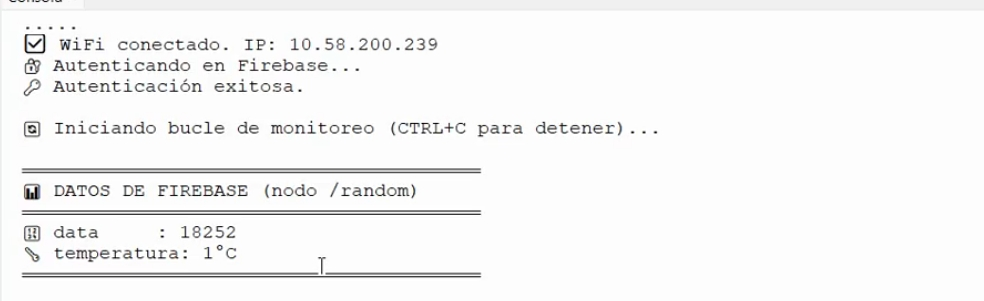
\includegraphics[width=0.8\textwidth]{FireBase/Salida.jpeg}
    \caption{Salida en el monitor serial de Thonny.}
\end{figure}

\end{document}
